\documentclass[14pt, a4paper]{report}
\usepackage[utf8]{inputenc}
\usepackage[russian]{babel}
\usepackage{multirow}
\usepackage{graphicx}
\renewcommand{\thesection}{\arabic{section}.}
\title{\textbf{Отчет о выполнении лабораторной работы 2.4.1 "Определение теплоты испарения жидкости"}}
\author{Калашников Михаил, Б03-205}
\date{}

\begin{document}

\maketitle

\textbf{Цель работы:} измерение давления насыщенного пара жидкости при разной температуре; вычисление по полученным данным теплоты испарения с помощью уравнения Клапейрона-Клаузиуса.
\newline

\textbf{Оборудование:} 
\begin{itemize}
  \item герметичный сосуд, заполненный испледуемой жидкостью;
  \item термостат ($\sigma_T=0,01\ K$);
  \item  отсчетный микроскоп ($\sigma_h=0,3\ mm$: погрешность микроскопа равна $0,1\ mm$, штангенциркуля -- $0,05\ mm$; прибор используется для нахождения разницы значений, погрешность удваивается).
\end{itemize}

\section{Теоретическая часть}

Теплота испарения жидкости может быть измерена непосредственно в процессе парообразования, однако такой метод оказывается неточен из-за потерь тепла. Другой метод, использующий формулу Клапейрона-Клаузиуса позволяет достичь большей точности. Данная формула связывает производную давления насыщенного пара $P$ по температуре $T$, теплоту испарения жидкости $L$, объем пара $V_2$ и объем жидкости $V_1$:
\[\frac{dP}{dT}=\frac{L}{T(V_2-V_1)}\]

При нашей точности опытов величиной $V_1$ можно пренебречь, а в виду того, что эксперимент проводится при пониженном давлении, можно принять газ за идеальный. Поэтому
\[V_2=\frac{RT}{P}\]

Подставляя это в формулу Клапейрона-Клаузиуса, получим:
\[L=\frac{RT^{2}}{P}\frac{dP}{dT}=-R\frac{d\left(\ln P\right)}{d\left(1/T\right)}\]

Таким образом, теплоту испарения можно найти как касательную к графику зависимости $\ln P$ от $1/T$, построенного с помощью метода наименьших квадратов.

С другой стороны, мы можем построить параболу через каждые три соседние точки на графике $P(T)$, провести к ней касательную и на основе этой касательной вычислить теплоту испарения. Далее усредним полученную теплоту испарения, а случаную погрешность определим как среднекватрическое отклонение.

В работе я попытаюсь определить теплоту парообразования обоими методами.

\section{Экспериментальная установка}

Лабораторная установка представлена на рис. 1. Установка включает термостат A, экспериментальный прибор B и отсчетный микроскоп C. 1 -- блок терморегулирования; 2 -- ванна; 3 -- индикаторное табло; 4 -- ручка установки температуры; 5 -- кнопка переключения режимов установки/контроля температуры; 6 -- индикатор уровня жидкости; 7 -- индикатор включения нагревателя; 8 -- сетевой выключатель прибора; 9 -- крышка; 10 -- входной и выходной патрубки насоса; 11 -- входной и выходной патрубки теплообменника (вода из водопровода). Экспериментальный прибор B представляет собой емкость 12, заполненную водой. В нее погружен запаянный прибор 13 с исследуемой жидкостью 14. Перед заполнением исследуемой жидкости воздух из запаянного прибора был удален, так что над жидкостью находится только её насыщенный пар. Давление пара определяется по ртутному манометру 15, соединенному с емкостью 13. Численная величина давления измеряется по разности показаний отсчетного микроскопа 16, настраиваемого последовательно на нижний и верхний уровни столбика ртути манометра. Показания микроскопа снимаются по шкале 17.

\begin{figure}[!ht]
\centering
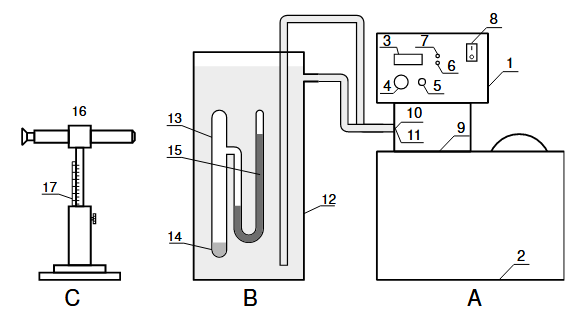
\includegraphics[scale=0.6]{terma_2_3.png}
\label{image3}
\caption{Схема установки}
\end{figure}

\section{Проведение эксперимента}

\begin{enumerate}
\item Измерим разность уровней ртути с помощью миркоскопа и температуру при выключенном термостате.

\item Включим термостат. Начнем постепенно нагревать газ, измеряя через каждый градус его высоту столбиков ртути с помощью отсчетного микроскопа. Для повышения надежности эксперимента каждое измерение было проведено трижды. При каждом измерении так же отметим температуру. Все полученные данные занесем в таблицу 1.

\item В ходе эксперимента термостат был нагрет с 20 до 38 градусов Цельсия. Провести измерения при охлаждении термостата не удалось ввиду нехватки времени.

\end{enumerate}

\section{Обработка данных}

\begin{enumerate}
\setcounter{enumi}{3}

\item Давление газа определяется формулой $P=\rho g\Delta h$, где $\Delta h=B-H$, $\rho$ -- плотность ртути, $g$ -- ускорение свободного падения ($\sigma_P=\rho_{Hg} g\sigma_h\approx40\ Pa$). По усредненным разностям высот найдем давление и занесем его в таблицу 2, а вычисленные значения $\ln P$ и $1/T$ -- в таблицу 3. Построим графиик зависимости $\ln P$ от $1/T$ (рис. 1) и $P(T)$ (рис. 2).

Проведем через точки таблицы 2 прямую с помощью метода наименьшего квадратов. Угловой коэффициент $k$ данной прямой позволяет вычислить теплоту испарения: $L=-Rk$.

Теперь найдем теплоту испарения с помощью второго метода. Для каждой касательной посчитаем теплоту и занесем в таблицу 4. По данным таблицы видно, что большой разброс данных не позволяет выделить зависимость $L(T)$.

\end{enumerate}

\section{Расчет погрешностей}

Теперь определим погрешность измерений.
В обоих способах расчета $L$ полная погрешность ищется по формуле:
\[\sigma_L=\sqrt{\sigma^2_{rand}+\sigma^2_{inst}}\]
Далее формулы для погрешности будут зависеть от метода обработки.
\newline\par
Первый метод.

Найдем случайную погрешность углового коэффициента проведенной прямой $\sigma_k$ и с помощью нее посчитаем случайную погрешность $L$:
\[\sigma_{rand}=R\sigma_k\]

Приборная погрешность определяется по формуле погрешности косвенных измерения:
\[\varepsilon_{inst, 1}=\sqrt{\varepsilon_{\Delta \ln P}^2+\varepsilon_{\Delta 1/T}^2}=2\sqrt{\varepsilon_{\ln P}^2+\varepsilon_{1/T}^2}=2\sqrt{\left(\frac{\sigma_{P}}{P\ln P}\right)^2+\left(\frac{\sigma_T}{T}\right)^2}=\]
\[=2\sqrt{<\frac{\varepsilon_{P}}{\ln P}>^2+<\varepsilon_{T}>^2}=0,3\%\]

В качестве $P$ и $T$ возьмем наименьшие соответсвующие значения из таблицы 2.

Второй метод:
Случайную погрешность $\sigma_{rand}$ определим как среднеквадратическое отклонение угловых коэффициентов касательных, а приборную аналогично с первым способом по формуле погрешности косвенных измерений:

\[\varepsilon_{inst, 2}=\sqrt{\varepsilon_P^2+4\varepsilon_T^2+\varepsilon_{\Delta P}^2+\varepsilon_{\Delta T}^2}=\sqrt{\left(\frac{\sigma_P}{P}\right)^2+4\left(\frac{\sigma_T}{T}\right)^2+\left(\frac{2\sigma_P}{P}\right)^2+\left(\frac{2\sigma_T}{T}\right)^2}=\]
\[=\sqrt{5<\varepsilon_P>^2+8<\varepsilon_T>^2}=2,7\%\]

\[\sigma_L=\sqrt{\sigma^2_{rand}+(\varepsilon_{inst}\cdot L)^2}\]

В результате обработки данных первым способом было получено значение $L_1=48,2\pm0,7\ \frac{kJ}{mol}$, а вторым $L_2=47\pm9\ \frac{kJ}{mol}$.

\section{Вывод}

Оба метода обработки данных дали примерно одинаковый результат, однако точность первого метода оказалась выше более чем на порядок. Полученное значение не сильно отличается от табличного, равного $41,4\ \frac{kJ}{mol}$.

\section{Приложения}
\begin{table}[!ht]
\centering
\makebox[\textwidth][c] {
\begin{tabular}{| c | c | c | c | c | c | c | c | c | c |}
\hline
$N$ & $t_1, ^\circ C$ & $B_1, mm$ & $H_1, mm$ & $t_2, ^\circ C$ & $B_2, mm$ & $H_2, mm$ & $t_3, ^\circ C$ & $B_3, mm$ & $H_3, mm$ \\
\hline
1	& 20,00	& 97,00	& 82,60	& 20,00	& 96,85	& 81,70	& 20,00	& 96,90	& 81,45 \\
2	& 21,00	& 97,15	& 81,40	& 21,00	& 97,05	& 81,85	& 21,00	& 96,75	& 81,75 \\
3	& 21,99	& 98,50	& 81,00	& 22,01	& 97,55	& 81,50	& 22,02	& 97,55	& 81,50 \\
4	& 23,01	& 97,95	& 81,10	& 23,01	& 98,15	& 80,70	& 23,00	& 97,95	& 80,70 \\
5	& 24,00	& 98,80	& 80,15	& 24,02	& 98,70	& 80,35	& 24,03	& 98,75	& 80,00 \\
6	& 25,05	& 99,35	& 79,65	& 25,06	& 99,75	& 79,65	& 25,07	& 99,55	& 79,65 \\
7	& 26,03	& 100,50	& 79,15	& 26,05	& 99,80	& 79,60	& 26,06	& 100,00	& 78,95 \\
8	& 27,04	& 101,30	& 77,80	& 27,05	& 101,50	& 77,95	& 27,08	& 101,45	& 78,10 \\
9	& 28,04	& 102,30	& 77,15	& 28,05	& 102,15	& 77,05	& 28,06	& 102,00	& 77,70 \\
10	& 29,06	& 103,10	& 76,20	& 29,07	& 102,70	& 76,65	& 29,08	& 103,20	& 76,45 \\
11	& 30,04	& 104,30	& 75,35	& 30,06	& 104,30	& 75,40	& 30,06	& 104,50	& 75,50 \\
12	& 31,06	& 104,95	& 74,55	& 31,06	& 105,00	& 75,00	& 31,06	& 104,85	& 74,90 \\
13	& 32,03	& 105,60	& 73,90	& 32,04	& 105,75	& 73,95	& 32,06	& 105,75	& 74,00 \\
14	& 33,04	& 106,40	& 72,70	& 33,05	& 106,70	& 73,00	& 33,05	& 106,60	& 72,60 \\
15	& 34,03	& 107,95	& 71,60	& 34,05	& 107,65	& 71,85	& 34,05	& 107,70	& 71,25 \\
16	& 35,05	& 109,00	& 70,40	& 35,05	& 108,70	& 70,60	& 35,05	& 109,00	& 70,80 \\
17	& 36,04	& 110,25	& 70,00	& 36,05	& 110,00	& 70,00	& 36,05	& 110,35	& 69,80 \\
18	& 37,04	& 110,70	& 69,00	& 37,04	& 110,50	& 68,70	& 37,05	& 110,40	& 69,15 \\
19	& 38,04	& 112,00	& 67,75	& 38,04	& 112,40	& 67,35	& 38,04	& 112,70	& 67,20 \\
\hline
\end{tabular}
}
\label{table1}
\caption{Измерения высот ртутных столбиков}
\end{table}

\begin{table}[!ht]
\centering
\begin{tabular}{| c | c | c | c | c | c | c | c |}
\hline
$T, K$ & $P, Pa$ & $T, K$ & $P, Pa$ &$T, K$ & $P, Pa$ & $T, K$ & $P, Pa$ \\
\hline
293,15	& 2150	& 298,21	& 2850	& 303,20	& 4150	& 308,20	& 5490 \\
294,15	& 2200	& 299,20	& 2990	& 304,21	& 4310	& 309,20	& 5770 \\
295,16	& 2370	& 300,21	& 3360	& 305,19	& 4550	& 310,19	& 5960 \\
296,16	& 2460	& 301,20	& 3560	& 306,20	& 4840	& 311,19	& 6440 \\
297,17	& 2660	& 302,22	& 3800	& 307,19	& 5190	& 	& \\
\hline
\end{tabular}
\label{table2}
\caption{Усреднение измеренных параметров}
\end{table}

\begin{table}[!ht]
\centering
\begin{tabular}{| c | c | c | c | c | c | c | c |}
\hline
$\frac{1}{T}, \frac{10^3}{K}$ & $lnP$ & $\frac{1}{T}, \frac{10^3}{K}$ & $lnP$ & $\frac{1}{T}, \frac{10^3}{K}$ & $lnP$ & $\frac{1}{T}, \frac{10^3}{K}$ & $lnP$ \\
\hline
3,41	& 7,67	& 3,35	& 7,96	& 3,30	& 8,33	& 3,24	& 8,61 \\
3,40	& 7,69	& 3,34	& 8,00	& 3,29	& 8,37	& 3,23	& 8,66 \\
3,39	& 7,77	& 3,33	& 8,12	& 3,28	& 8,42	& 3,22	& 8,69 \\
3,38	& 7,81	& 3,32	& 8,18	& 3,27	& 8,49	& 3,21	& 8,77 \\
3,37	& 7,89	& 3,31	& 8,24	& 3,26	& 8,55	& 	& \\
\hline
\end{tabular}
\label{table3}
\caption{Обработка усредненных параметров}
\end{table}

\begin{table}[!ht]
\centering
\begin{tabular}{| c | c | c | c | c | c |}
\hline
$T, K$ & $L, kJ/mol$ & $T, K$ & $L, kJ/mol$ & $T, K$ & $L, kJ/mol$ \\
\hline
294,15	& 36	& 300,21	& 63	& 306,20	& 51 \\
295,16	& 40	& 301,20	& 47	& 307,19	& 49 \\
296,16	& 43	& 302,22	& 59	& 308,20	& 42 \\
297,17	& 53	& 303,20	& 48	& 309,20	& 33 \\
298,21	& 42	& 304,21	& 36	& 310,19	& 45 \\
299,20	& 63	& 305,19	& 45	& 	& \\
\hline
\end{tabular}
\label{table4}
\caption{Величины $L$, найденные вторым методом обработки}
\end{table}


\begin{figure}[!ht]
\centering
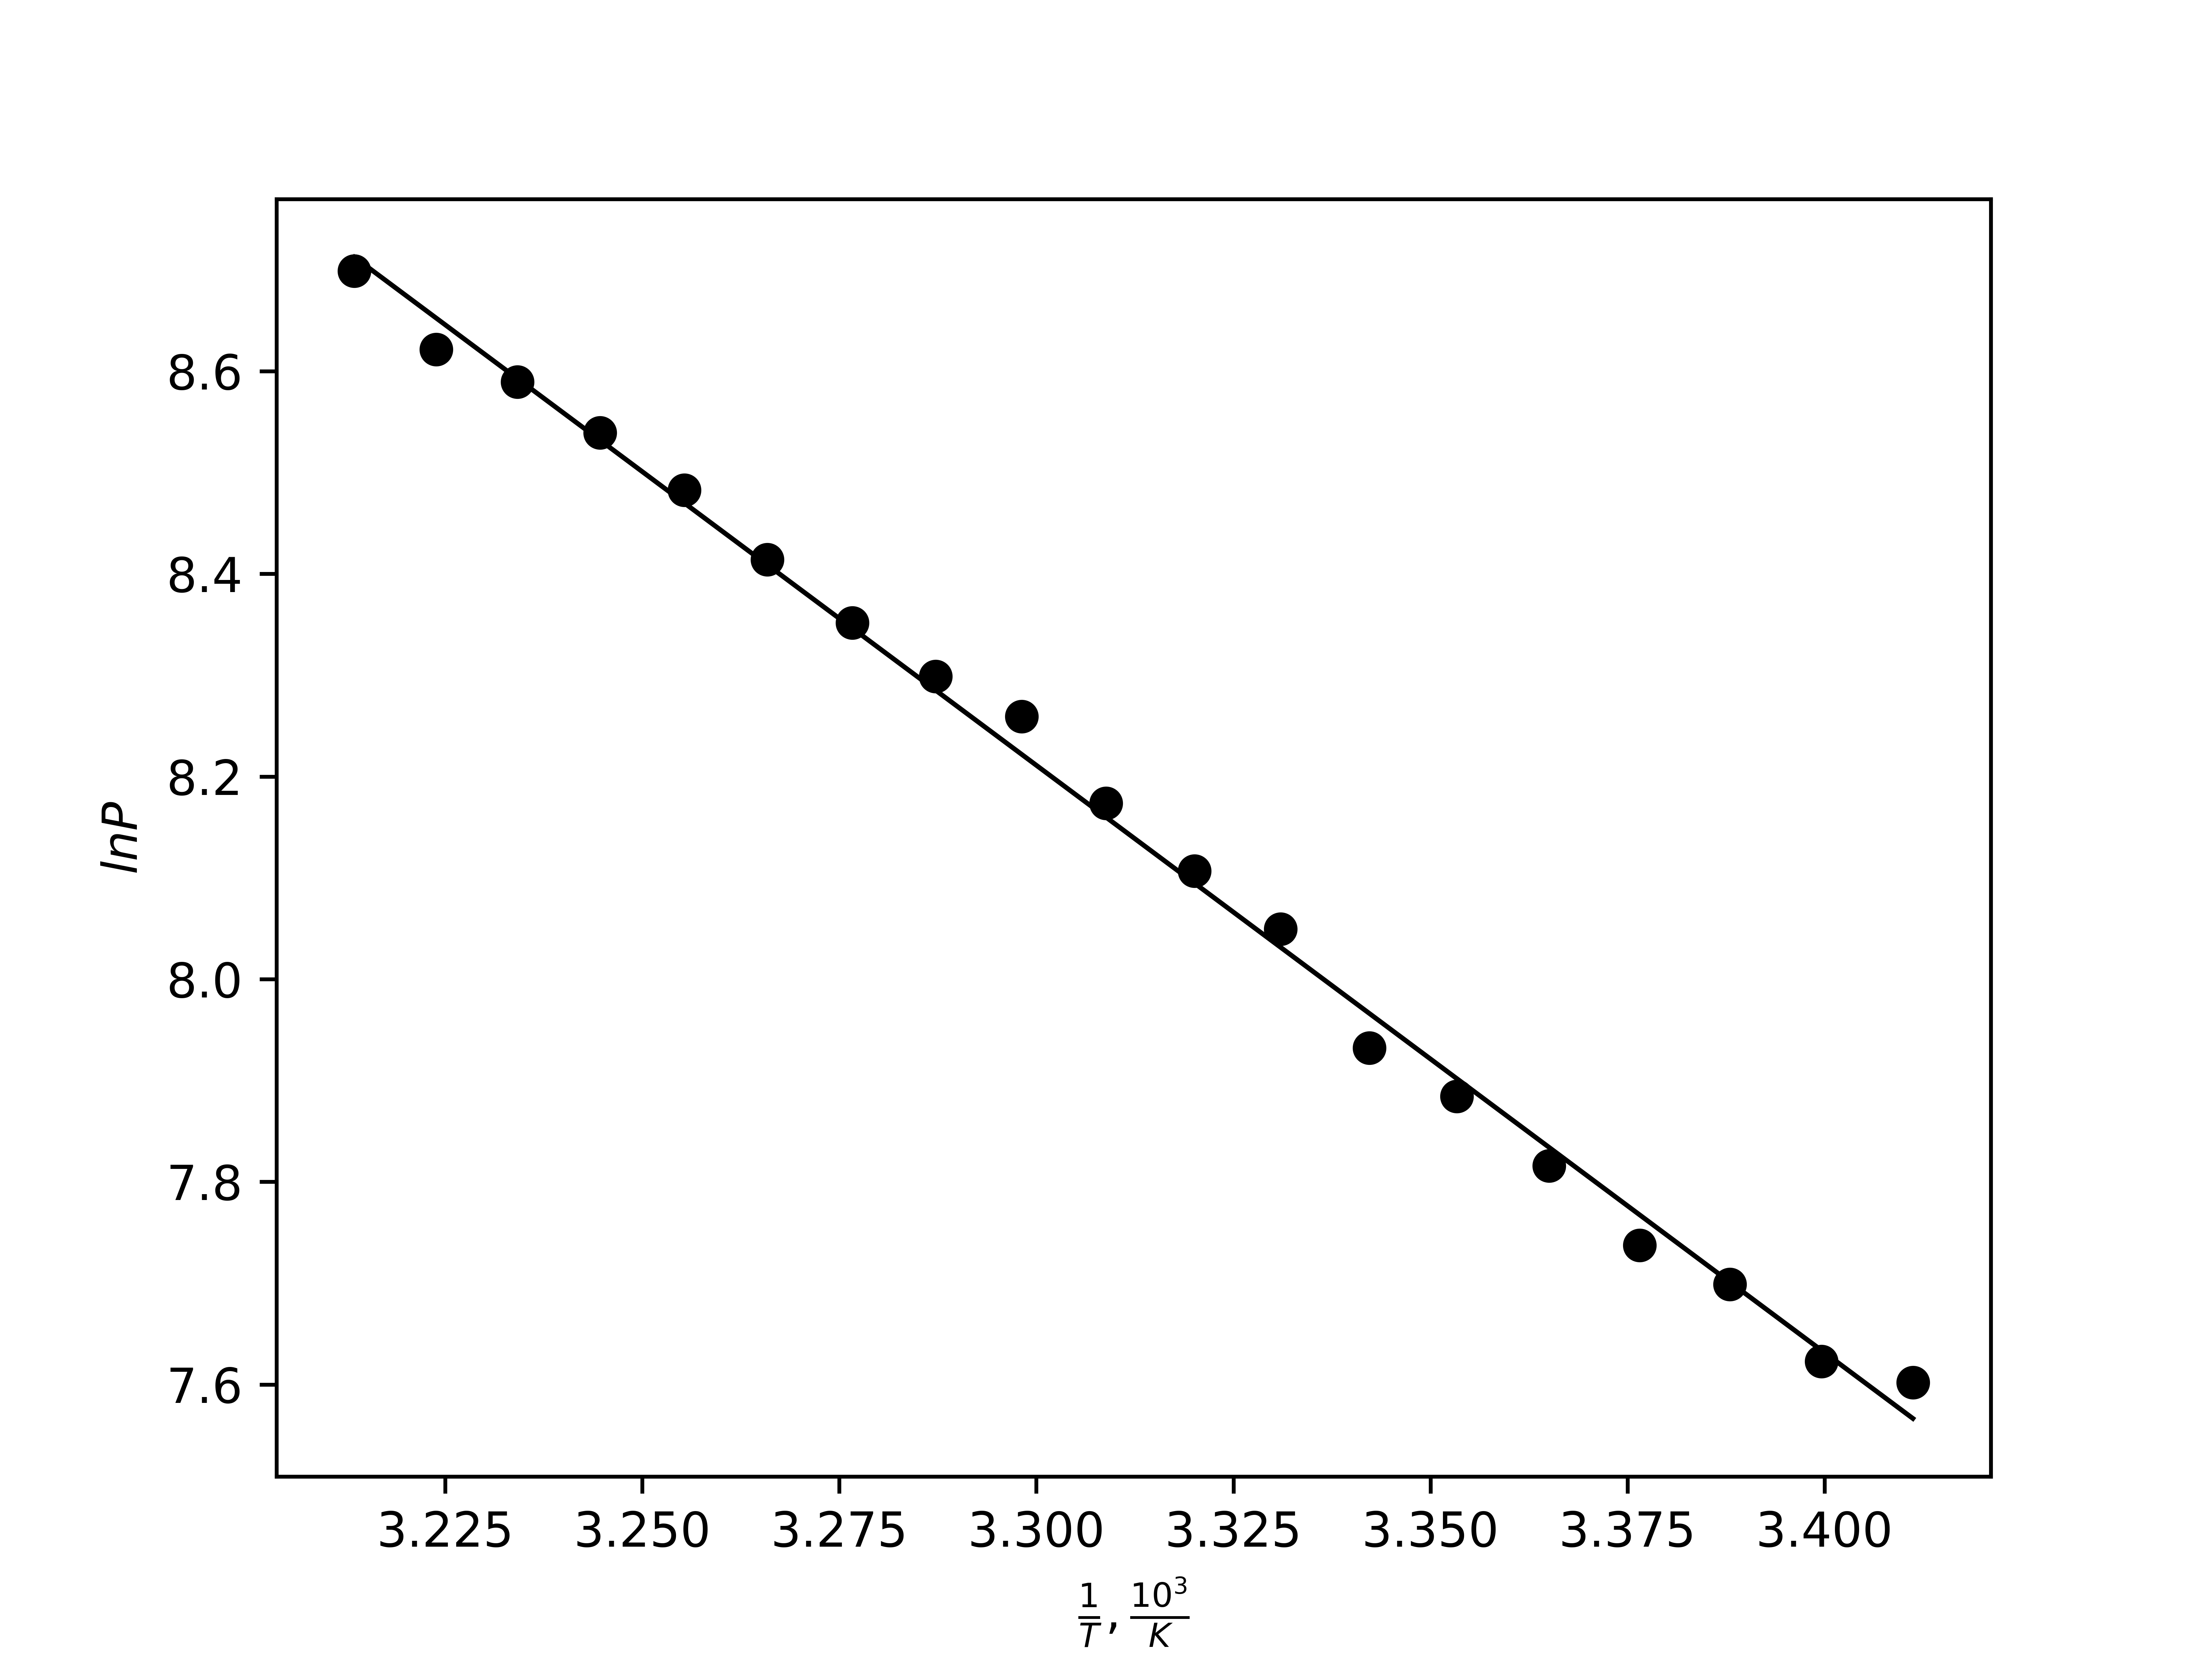
\includegraphics[scale=0.8]{terma2_1.png}
\label{image1}
\caption{График зависимости $\ln P$ от $1/T$}
\end{figure}

\begin{figure}[!ht]
\centering
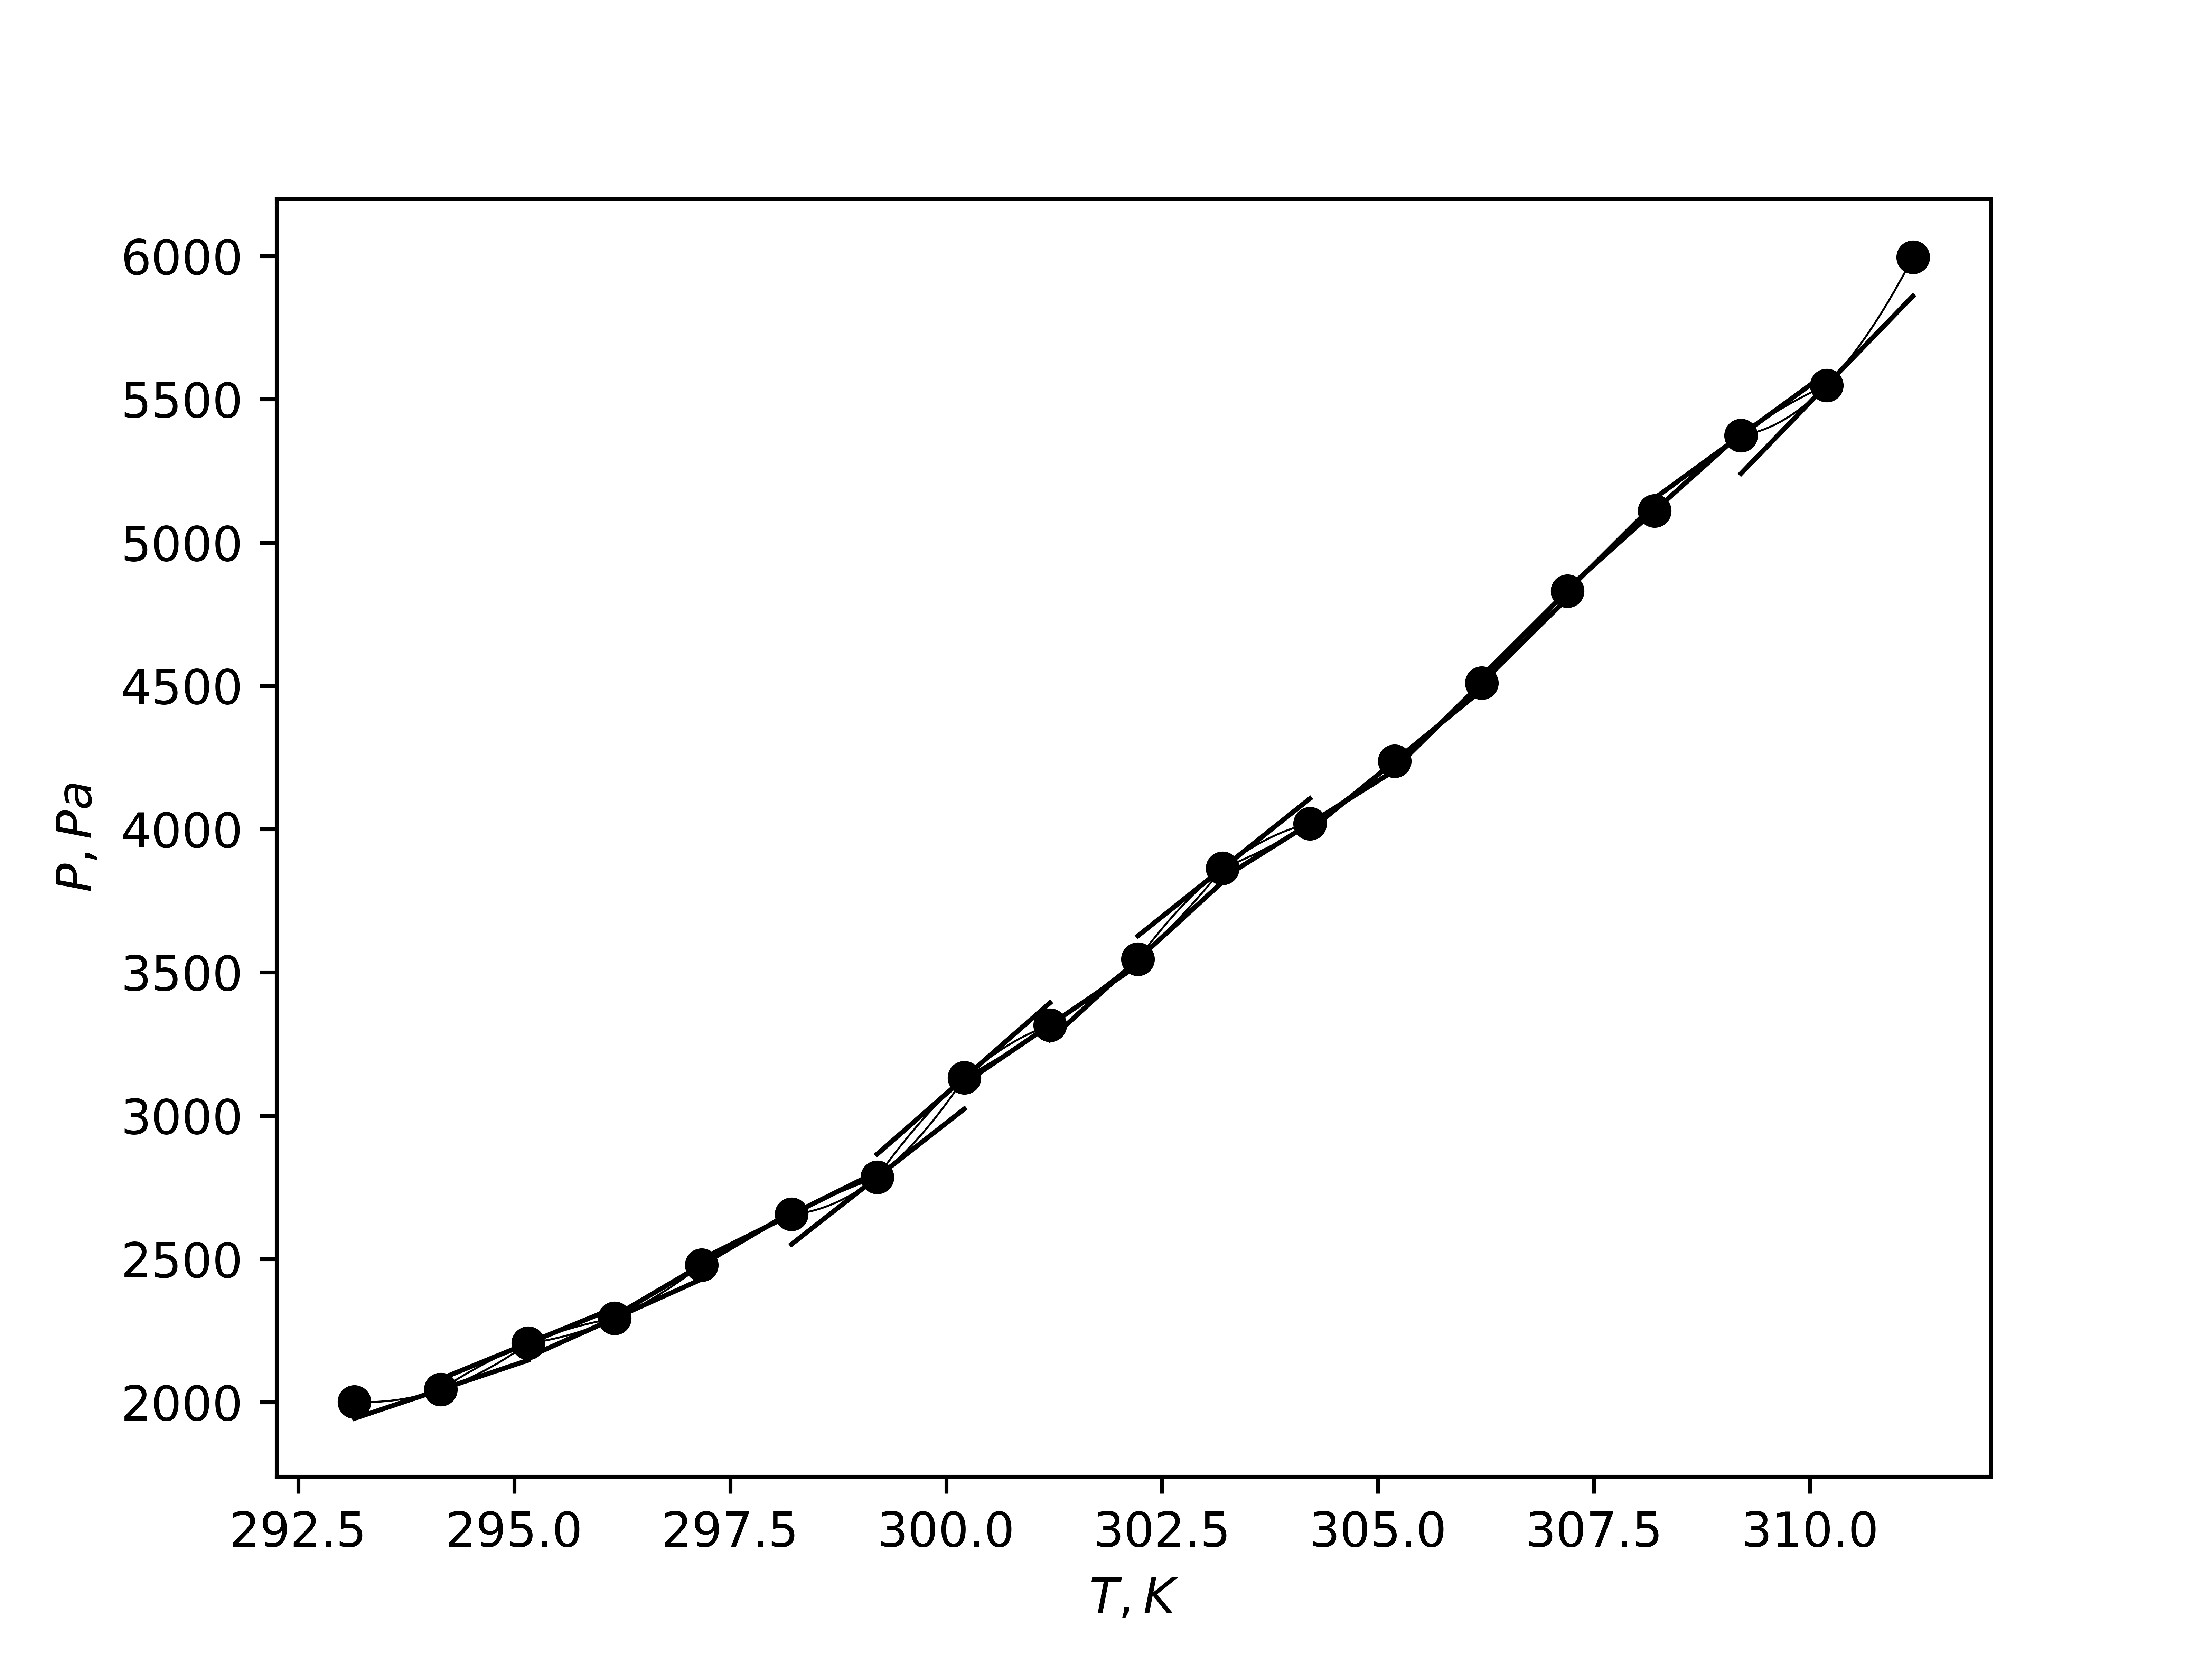
\includegraphics[scale=0.8]{terma2_2.png}
\label{image2}
\caption{График зависимости $P(T)$}
\end{figure}


\end{document}